\documentclass[aps,pre,preprint]{revtex4}
% \documentclass[aps,jcp,groupedaddress,twocolumn,unsortedaddress]{revtex4}

\usepackage{amsmath}
\usepackage{amssymb}
\usepackage[dvips]{graphicx}
\usepackage{color}
\usepackage{tabularx}

\makeatletter
\makeatother

\newcommand{\recheck}[1]{{\color{red} #1}}
\renewcommand{\v}[1]{\textbf{\textit{#1}}}
\renewcommand{\d}[1]{\textsf{#1}}


\begin{document}

\title{The Error Estimate of Force Calculation in Heterogeneous and Correlated Molecular Systems}
\author{Han Wang}
\affiliation{LMAM and School of Mathematical
  Sciences, Peking University}
\author{Pingwen Zhang}
% \email{pzhang@pku.edu.cn}
\affiliation{LMAM and School of Mathematical
  Sciences, Peking University}

\begin{abstract}
\end{abstract}

\maketitle

\section{Theoretical background}
\subsection{Error estimate in a heterogeneous system}

If a particle with cut-off radius $r_c$ is located at position $\v r$,
we denote the computed force (or cut-offed force) by $\tilde{\v F}(\v
r)$. The difference between the exact force and the computed force,
namely the error force, is denoted by $\Delta\v F(\v r) = \v F(\v r) -
\tilde{\v F}(\v r)$. The error force can be expressed by
\begin{align}
  \Delta\v F(\v r) = \sum_{j}\, \v f^c(\v r - \v r_j)
\end{align}
where $\v f^c$ is the complementary pairwise short-range force defined
by
\begin{align}
  \v f^c(\v r) =
  \left\{
  \begin{array}{ll}
    0, & \vert\v r\vert\leq r_c; \\
    \v f(\v r), & \vert\v r\vert > r_c.
  \end{array}
  \right.
\end{align}
In a homogeneous system with periodic boundary condition applied, the
surounding of any particle is isotropic, so the mean of the error
force vanishes. However, in a heterogenous system, the mean of the
error force is not necessarily zero, but
\begin{align} \label{eqn:tmp3} %\nonumber
  \langle\Delta\v F(\v r)\rangle
  &=
  \big\langle
  \sum_{j}\, \v f^c(\v r - \v r_j)
  \big\rangle 
  =
  \int_{\mathbb R^3}\v f^c(\v r - \v r')\rho(\v r')\,\d d\v r'
\end{align}
Where $\rho(\v r)$ is the particle number density at the position $\v
r$. And notice the error force implicitly depends on the cut-off
radius used for the particle.

The widely accepted definition of the force error is the root mean
square (RMS) error, namely the square root of the second moment of the
error force is $\mathcal E(\v r) = \sqrt{\langle\vert\Delta\v F(\v
  r)\vert^2\rangle}$, which can be calculate by
\begin{align} \nonumber
  \langle\vert\Delta\v F(\v r)\vert^2\rangle
  =\,&
  \big\langle\sum_{j,k}\v f^c(\v r - \v r_j)\cdot\v f^c(\v r - \v r_k)\big\rangle \\ \nonumber
  =\,&
  \big\langle\sum_j\vert\v f^c(\v r - \v r_j)\vert^2\big\rangle +
  \big\langle\sum_{j\neq k}\v f^c(\v r - \v r_j)\cdot\v f^c(\v r - \v r_k)\big\rangle \\ \nonumber
  =\,&
  \int_{\mathbb R^3}\vert\v F^c(\v r - \v r')\vert^2\rho(\v r')\,\d d\v r'
  + \\\label{eqn:tmp4}
  \,&
  \int_{\mathbb R^3\times\mathbb R^3}\v F^c(\v r - \v r')\cdot\v F^c(\v r - \v r'')\rho(\v r', \v r'')\,\d d\v r'\d d\v r'',
\end{align}
The density $\rho(\v r')$ and the pair density $\rho(\v r', \v r'')$
are related to the probability density $p(\v r')$ and pair probability
density $p(\v r', \v r'')$ by
\begin{align}
  \rho(\v r') &= N\,p(\v r') \\
  \rho(\v r', \v r'') &= N(N-1)\,p(\v r', \v r'')
\end{align}
The densities are periodically extented to the whole space $\mathbb
R^3$.
% The problem now this how to discretize the integrals in
% \eqref{eqn:tmp4}. With the piecewise constant numerical integration
% formulus, we have:
Now, let
\begin{align} \nonumber
  \rho(\v r', \v r'')
  & = N (N-1) \,p(\v r', \v r'') \\\nonumber
  & = N (N-1) \big\{ p(\v r')p(\v r'') + [\,p(\v r', \v r'') -  p(\v r')p(\v r'')\,]\big\} \\\nonumber
  &= \frac{N-1}N \rho(\v r')\rho(\v r'') + C (\v r', \v r'')\\ \label{eqn:tmp7}
  &\approx \rho(\v r')\rho(\v r'') + C (\v r', \v r'')
\end{align}
the function
\begin{align}
C (\v r', \v r'') = N (N-1) [\,p(\v r', \v r'') -  p(\v r')p(\v r'')\,]
\end{align}
denotes the correlation between
position $\v r'$ and $\v r''$. Therefore, \eqref{eqn:tmp4} becomes
\begin{align} \nonumber
  \langle\vert\Delta\v F(\v r)\vert^2\rangle
  = &\,
  \int_{\mathbb R^3}\vert\v f^c(\v r - \v r')\vert^2\rho(\v r')\,\d d\v r' \,+ \\\nonumber
  &\,
  \bigg[\int_{\mathbb R^3}\v f^c(\v r - \v r')\rho(\v r')\,\d d\v r'\,\bigg]^2 + \\\nonumber
  &\,
  \int_{\mathbb R^3\times\mathbb R^3}\v f^c(\v r - \v r')\cdot\v f^c(\v r - \v r'')\,C(\v r', \v r'')\,\d d\v r'\d d\v r'' \\\label{eqn:tmp5}
  = &\,
  \mathcal E_{\textrm{homo}}(\v r) +
%  \langle\Delta\v F(\v r)\,\rangle^2 +
  \mathcal E_{\textrm{hetero}}(\v r) +
  \mathcal E_{\textrm{correlation}}(\v r)
\end{align}
If the system is homogeneous and the correlation between particles is
neglected, then only the first term, which is called the homogeneity
error, is left in \eqref{eqn:tmp5}. This term is originated from the
flucuation of the error force $\Delta\v F(\v r)$. The second term is
called the heterogeneity error, because it only exists when the system
is heterogenous. It is worth poining out that the heterogeneity error
is the squared mean of the error force, namely $\mathcal
E_{\textrm{hetero}}(\v r) = \langle\Delta\v F(\v r)\,\rangle^2$.  The
last term in \eqref{eqn:tmp5} originates from the correlation between
the particles, so it is called the correlation error.  The correlation
error involves a double integrals, which implies that this term
requires more compuational cost than the homogeneity and heterogeneity
errors. The rest of this paper assumes the system is far from the
critical point, therefore the correlation error does not dominate in the
system, and can be savely neglected.


\subsection{The ways to reduce force error in a heterogenous system}

In Fig. \ref{fig:tmp1}, the testing system containing $N=16000$
standard Lennard-Jone particles is set up in a tube with periodic
boundary condition. The liquid droplet (in the middle of the tube) is
in equilibrium with the surrounding vapor environment. The red line in
the Fig. \ref{fig:tmp2} denotes the density profile (on direction $x$)
of this heterogeneous system. The green square denotes the real RMS
force error distribution. It is clear that the error form two peaks in
the interfacial region, which is much higher than the relative
constant error of the bulk liquid and the bulk vapor. The dashed and
the dotted blue line are the estimated homogeneity and heterogeneity
errors, and the solid blue line is the sum. In the bulk region, the
homogeneity error dominates while in the interfacial region, the
heterogeneity error dominates. The esitmated error matches perfactly
with the real error at the interfacial region, but presents
overestimation in the bulk regions. The overestimation probably stems
from the neglection of the correlation error in \eqref{eqn:tmp5}.

Traditionally, a very large cutoff radius is used to reach precise
simulation results. Since heterogeneity error dominate the force error
of the system, such a big cutoff radius is a waste in the bulk liquid
and vapor regions. One possible way is to use adapt cut-off radius
according to the error distribution, so that larger cut-off radii are
used in the interfacial region while smaller cut-off radii are used in
the bulk regions.  More precisely, the aim of the adaptive cut-off
method is to equivalently distributed the force error over the
simulation region.

The other way is to screen out the heterogeneity error by a applying a
correction force.  Starting from equation \eqref{eqn:tmp5}, the
variation of the error force can be calculated by
\begin{align} \nonumber
  \textrm{Var}[\Delta\v F(\v r)]
  & =
  \big\langle\,
  [\,\Delta\v F(\v r) - \langle\Delta\v F(\v r)\rangle\,]^2
  \big\rangle \\\nonumber
  & =
  \langle\vert\Delta\v F(\v r)\vert^2\rangle -
  \langle\Delta\v F(\v r)\,\rangle^2 \\
  & =
  \mathcal E_{\textrm{homo}}(\v r) +
  \mathcal E_{\textrm{corr}}(\v r)  
\end{align}
This means if we correct the computed force by the mean of the error
force, namely applying to each particle $\tilde{\v F}^c(\v r) =
\tilde{\v F}(\v r) - \langle\Delta\v F(\v r)\rangle$ instead of
$\tilde{\v F}(\v r)$. The error of this corrected force is reduced to
$\mathcal E_{\textrm{homo}}(\v r) + \mathcal E_{\textrm{corr}}(\v r)$
and contains no heterogeneous contribution.  These two possibilities
will be addressed and tested later in this paper.

% This
% means the force error is a combination of a homogeneous contribution,
% a heterogeneous contribution and a correlational contribution. The
% heterogeneous force can be applied as a correction to the error:
% \begin{align}\label{eqn:tmp7}
%   \v F_{\textrm{hetero}} = \int_{\mathbb R^3}\v F^c(\v r - \v r')\rho(\v r')\,\d d\v r'
% \end{align}

\subsection{The fast calculation of the error estimate}\label{sec:tmp1.3}

The fast calculation of the convolutions in \eqref{eqn:tmp5} relies on
the fast Fourier transform. We assume the simulation box is uniformly
divided in to small bins.  The positions of these bins are
\begin{align}
  \v r_{i_1, i_2, i_3} & =
  \frac{i_1}{K_1}\v a_1 + 
  \frac{i_2}{K_2}\v a_2 + 
  \frac{i_3}{K_3}\v a_3,\qquad 0\leq i_\alpha< K_\alpha
\end{align}
where $\v a_\alpha$ are box vectors, and $K_\alpha$ is the number of
division on each direction. In the reciprocal space, a corresponding
lettice is set up:
\begin{align}
  \v k_{k_1, k_2, k_3} & =
  k_1\v a_1^\ast +
  k_2\v a_2^\ast +
  k_3\v a_3^\ast, \qquad 0\leq k_\alpha<K_\alpha
\end{align}
where $\v a_\alpha^\ast$ are reciprocal box vectors defined by $\v
a_\alpha\cdot\v a_\beta^\ast = \delta_{\alpha\beta}$.  In each bin the
error and the particles number density are assumed to be constant,
therefore,
\begin{align}\nonumber
  \mathcal E_{\textrm{homo}}(\v r_{i_1,i_2,i_3})
  & \approx
  \frac1V\sum_{k_1=-\infty}^\infty\sum_{k_2=-\infty}^\infty\sum_{k_3=-\infty}^\infty
  \hat{\mathcal E}_{\textrm{homo}}(\v k_{k_1,k_2,k_3})
  % e^{2\pi i\v k_{k_1,k_2,k_3}\cdot\v r_{i_1,i_2,i_3}}
  \exp\bigg[
  2\pi i\bigg(
  \frac{k_1i_1}{K_1} + \frac{k_2i_2}{K_2} + \frac{k_3i_3}{K_3}
  \bigg)
  \bigg] \\\label{eqn:tmp13}
  & \approx
  \frac1V\sum_{k_1=0}^{K_1}\sum_{k_2=0}^{K_2}\sum_{k_3=0}^{K_3}
  \hat{K}_{\textrm{homo}}(\v k'_{k_1,k_2,k_3})\:
  \hat{\rho}(\v k_{k_1,k_2,k_3})
  % e^{2\pi i\v k_{k_1,k_2,k_3}\cdot\v r_{i_1,i_2,i_3}}
  \exp\bigg[
  2\pi i\bigg(
  \frac{k_1i_1}{K_1} + \frac{k_2i_2}{K_2} + \frac{k_3i_3}{K_3}
  \bigg)
  \bigg]   
\end{align}
here we denote the convolution kernel $\vert\v f^c(\v r)\vert^2$ by
$K_{\textrm{homo}}(\v r)$.  Equation \eqref{eqn:tmp13} simply utilizes
the identity: the Fourier transform of the convolution
$K_{\textrm{homo}}\ast\rho$ is equal to the multiply of
$\hat{K}_{\textrm{homo}}$ and $\hat\rho$.  The prime on $\v
k_{k_1,k_2,k_3}$ means that we should use the periodic image $k_\alpha
- K_\alpha$ instead of $k_\alpha$ when $k_\alpha \geq K_\alpha/2$. By
definition, the Fourier transform of the density is
\begin{align}
  \hat\rho(\v k_{k_1,k_2,k_3})
  & \approx
  \frac{V}{K_1K_2K_3}
  \sum_{i_1=0}^{K_1}\sum_{i_2=0}^{K_2}\sum_{i_2=0}^{K_2}
  \rho(\v r_{i_1,i_2,i_3})
  \exp\bigg[
  -2\pi i\bigg(
  \frac{k_1i_1}{K_1} + \frac{k_2i_2}{K_2} + \frac{k_3i_3}{K_3}
  \bigg)
  \bigg]
\end{align}
The Fourier transform of the homogeneity kernel is 
\begin{align}
  \hat K_{\textrm{homo}}(\v k)
  &=
  \int_{\mathbb R^3}K_{\textrm{homo}}(\v r)e^{-2\pi i\v k\cdot\v r}\,\d d\v r
\end{align}
Most of the short-range interactions are isotropic, therefore,
$K_{\textrm{homo}}(\v r) = K_{\textrm{homo}}(r)$, and
\begin{align}
  \hat{K}_{\textrm{homo}}(\v k)
  =
  \int_{\mathbb R^3}K_{\textrm{homo}}(r)e^{-2\pi i\v k\cdot\v r}\d d\v r
  =
  \int_{r_c}^\infty \frac{2 r}k\, K_{\textrm{homo}}(r) \sin(2\pi kr)\,\d dr
\end{align}


Similarly, by \eqref{eqn:tmp3}, the Fourier mode of the the mean of
the error force is
\begin{align}
  \langle\Delta\v F\rangle^\wedge(\v k) =
  \hat{\v f}^c(\v k)\,
  \hat\rho(\v k)
\end{align}
where 
\begin{align}\label{eqn:tmp18}
  \hat{\v f}^c(\v k) 
  & = 
  2\pi\frac{\v k}k\, i\,
  \bigg\{
  r_c^2\,u(r_c)
  \bigg[\,
  \frac{2\cos(2\pi kr)}{2\pi kr}
  -\frac{2\sin(2\pi kr)}{(2\pi kr)^2}
  \,\bigg] 
  -
  \int_{r_c}^\infty 2r\,u(r)\sin(2\pi kr)\d d\v r
  \bigg\}
\end{align}


\subsection{Pressure corrections}
By cut-off method, the system lost the  pressure
contribution from the particles outside the cut-off radius.  In the
homogeneous systems, the distribution of particles is assumed to be
uniform and the energy and pressure corrections are calculated by
integral corresponding pair functions from the cut-off to infinity.

In the heterogeneous systems, the previous idea does not
work. Instead, the pressure correction of the
system are:
\begin{align}
  \v P^c &= \frac1{V} \bigg\langle \sum_{i\neq j}\,\frac12\, (\v r_i - \v r_j) \otimes \v f^c(\v r_i - \v r_j) \bigg\rangle
\end{align}
For simplicity, let us consider the general form the the corrections:
\begin{align}
  Q = \bigg\langle \sum_{i\neq j} K(\v r_i - \v r_j) \bigg\rangle
\end{align}
For the pressure correction, $K$ is replaced by $\frac{1}{2V}\v
r\otimes\v f^c$.  By using \eqref{eqn:tmp7}, we have
\begin{align}\nonumber
  Q
  &= \bigg\langle \sum_{i\neq j} K(\v r_i - \v r_j) \bigg\rangle\\\nonumber
  & = \int K(\v r' - \v r'') \rho(\v r', \v r'') \d d\v r'\d d\v r'' \\\nonumber
  & = \int K(\v r' - \v r'')
  \big[
  \rho(\v r') \rho(\v r'') + C(\v r', \v r'')
  \big]
  \d d\v r'\d d\v r''
\end{align}
Assuming the correlation $C(\v r', \v r'')$ vanishes, then
\begin{align} \nonumber
  Q 
  & = \int K(\v r' - \v r'')
  \rho(\v r') \rho(\v r'') 
  \d d\v r'\d d\v r'' \\
  & = \int
  \Big[
  \int K(\v r' - \v r'') \rho(\v r'')\,\d d\v r''
  \Big]
  \rho(\v r')\,\d d\v r'
\end{align}

The Fourier transform of the convolution $\int K(\v r' - \v r'')
\rho(\v r'')\,\d d\v r''$ is identical to the product $\hat K(\v
k)\,\hat \rho(\v k)$. In the case of pressure correction, the Fourier
transform of $\frac{1}{2V}\v r\otimes\v f^c$ requires more efforts.
For the isotropic short-range interactions, the $\alpha\beta$
component of the pressure correction kernel can be written as
\begin{align}
  \frac1{2V}\{\v r\otimes\v f^c\}_{\alpha\beta} =
  r_\alpha r_\beta \,G^c(r) \qquad \alpha, \beta = 1, 2, 3
\end{align}
where $G^c(r)$ is independent with the direction of $\v r$.  We list
here without proving the Fourier transform of the pressure correction
kernel:
\begin{align}
  [\,r_1r_1\,G^c(r)\,]^{\wedge} 
  =\,& 
  \int_{r_c}^\infty \d dr\, r^4 G(r)\,
  \pi \sqrt{ \frac1{kr} }\,
  \Big[\,
  \frac23\,J_{\frac12}(2\pi kr) -
  \big(\,
  \frac13 -
  \cos^2\Phi +
  \sin^2\Phi\cos2\Theta
  \big)\, J_{\frac52}(2\pi kr)
  \,\Big] \\
  [\,r_2 r_2\,G^c(r)\,]^{\wedge} 
  =\,& 
  \int_{r_c}^\infty \d dr\, r^4 G(r)\,
  \pi \sqrt{ \frac1{kr} }\,
  \Big[\,
  \frac23\,J_{\frac12}(2\pi kr) -
  \big(\,
  \frac13 -
  \cos^2\Phi -
  \sin^2\Phi\cos2\Theta
  \big)\, J_{\frac52}(2\pi kr)
  \,\Big]   \\
  [\,r_3 r_3\,G^c(r)\,]^{\wedge} 
  =\,& 
  \int_{r_c}^\infty \d dr\: \,r^4 G(r)\,\pi\,
  \sqrt{ \frac1{kr} }\,
  \Big[\,
  \frac23 J_{\frac12}(2\pi kr) +
  \big(\,
  \frac23 - 2\cos^2\Phi
  \big)
  J_{\frac52}(2\pi kr)
  \,\Big]\\
  [\,r_1 r_2\,G^c(r)\,]^{\wedge} 
  =\,& -
  \int_{r_c}^\infty
  \d dr\,
  r^4G(r)\,\pi\,
  \sqrt{\frac1{kr}}\:
  \sin^2\Phi\sin 2\Theta\,J_{\frac52}(2\pi kr)\\
  [\,r_1 r_3\,G^c(r)\,]^{\wedge} 
  =\,& -
  \int_{r_c}^\infty
  \d dr\,
  r^4G(r)\,\pi\,
  \sqrt{\frac1{kr}}\:
  \sin2\Phi\cos\Theta\,J_{\frac52}(2\pi kr)\\
  [\,r_2 r_3\,G^c(r)\,]^{\wedge} 
  =\,& -
  \int_{r_c}^\infty
  \d dr\,
  r^4G(r)\,\pi\,
  \sqrt{\frac1{kr}}\:
  \sin2\Phi\sin\Theta\,J_{\frac52}(2\pi kr)
\end{align}
Where $(k, \Phi, \Theta)$ are the spherical coordinates of reciprocal
variable $\v k$, and $J_\nu(x)$ is the Bessel function of the first
kind.


\subsection{Details on implementing the adaptive cut-off radius
  method}

The adaptive cut-off radius method should be able to choose a proper
cut-off radius for each particle so that the force error is below a
predetermined target precision $\mathcal E^\ast$. The computational
cost of this operation is at least $\mathcal O(N^2\log N)$.  Becasue
to determine the cut-off radius, we should estimate the force error at
least once for each particle, and the computational cost of the force
error estimate \eqref{eqn:tmp5} is $\mathcal O(N \log N)$.

To reduce the computational cost, we assume
\begin{enumerate}
\item The space is divided in to small bins, the size of which is the
  same as those mentioned in the section \ref{sec:tmp1.3}. The cut-off
  radius is assumed to be constant within a bin, no matter the
  position of the partile.
\item The cut-off radius can only be set to a series of increasing
  discrete values between a maximum cut-off radius
  $r_c^{\textrm{max}}$ and a minimum cut-off radius
  $r_c^{\textrm{min}}$, namely $\{\,r_c^{\textrm{min}} = r_c^0 <
  r_c^1 < \cdots < r_c^{M-1} <r_c^M = r_c^{\textrm{max}}\}$. For
  convenience but not necessarily, the interval between two neighboring
  cut-off radius in uniform, which means
  \begin{align}
    r_c^m = r_c^0 + r_c^{\textrm{step}} m, \quad 0 \leq m \leq M
  \end{align}
  For example in some
  simulation cases, we set $r_c^{\textrm{max}} = 10.0\sigma$ and
  $r_c^{\textrm{min}} = 2.5\sigma$. In between the cut-off radius is
  adapted at a step of $0.5\sigma$, namely can only use values such as
  $2.5\,\sigma,\ 3.0\,\sigma,\ 3.5\,\sigma,\ 4.0\,\sigma,\ \cdots,\
  10.0\,\sigma$. 
\end{enumerate}

For each cut-off radius, the force error distribution $\mathcal E(\v
r)$, which is also defined on the lattice, is calculated by estimate
\eqref{eqn:tmp5}. Then a satisfactory cut-off radius of a bin is
choosen such that it is the smallest one that satisfying the precision
constrain $\mathcal E(\v r_{i_1,i_2,i_3}) \leq \mathcal E^\ast$. The
computational cost of this algorithm is $\mathcal O(MN\log N)$.  The
idea of this algorithm is based on the observation that the cut-off
radius may not be calculated at a high precision, a slightly (and at
most $r_c^{\textrm{step}}$) larger cut-off radius will not waste too
much computational cost.




\section{Results and discussions}

\subsection{Liquid-vapor coexistence simulation of the Lennard-Jones fluid}\label{sec:tmp2.1}

The liquid-vapor coexistence simulation is a very typical
heterogeneous molecular system, which is widely used to study the
phase coexistence properties, for example, the equilibrium liquid and
vapor density, and the surface tension. The system contains 16,000
standard Lennard-Jones particles that saperated into liquid phase in
the center of the box and vapor phase surrounded. The size of the
simulation box is $L_x^\ast \times \L_y^\ast \times L_z^\ast =
150\times 21\times 21$. This simulation box permit a maximum cut-off
radius of $r_c^\ast = 10$, and eliminate the finite scale effect
discussed in literatures \recheck {give citations here}. In all
simulations, the maximum cut-off radius considered is $10$, but the
reference (precise value) results are given by a simulation carried
out in a 24,000 particles system with simulation box $L_x^\ast \times
\L_y^\ast \times L_z^\ast = 150\times 27\times 27$, and a uniform
cut-off radius of $r_c^\ast = 13$.

Figure \ref{fig:tmp2} presents the real RMS force error (in green
square) in a system using a uniform cut-off raidus of $r_c^\ast =
7.5$. The number density distribution along $x$ direction that is
shown by the solid red line for reference.  The error is comparatively
constant at the bulk liquid and gas region and two paaks, which are
more than one order of maganitude higher than the bulk force errors,
form at the interfacial region.  The estimated RMS force error is
presented in solid blue line.  The estimate follows the real error
very well at the interfacial region, but slightly over estimate the
error in the bulk regions.  Two component of interest, namely the
homogeneous error and heterogeneous error are presented in
Fig. \ref{fig:tmp2} by dashed and dotted blue lines, respectively.  In
the bulk regions, the dashed blue line overlaps with the solid blue
line, that means the homogeneous error dominates.  In the interfacial
region, in the contrary, the heterogeneous error dominate, because the
dotted blue line overlaps with the solid one.

The Fig. \ref{fig:tmp2} inspire us to develop the adaptive cut-off
method: in the bulk regions, the error is much smaller, therefore, it
is a waste to use the same cut-off radius in the bulk as the
interfacial region. The key idea is to use small cut-off radius in the
bulk regions, so that the RMS force error is uniformly distributed
over the simulation region. In Fig. \ref{fig:tmp3}, we present the
adapted cut-off radius in a solid red line and all errors in the same
notation as the Fig. \ref{fig:tmp2}. The control error $\mathcal
E^\ast = 0.0045$ is the same as the maximum error in the uniform
cut-off simulation. In the interfacial region, the cut-off radius used
is the same as in Fig. \ref{fig:tmp2}, namely $7.5$.  Whereas, in the
liquid and vapor regions, the cut-off radii are $4.75$ and $3.5$,
respective, which is notably reduced. Considering the computational
cost grows with $r_c^3$, the adaptive simulation save 75 \% and 90 \%
computational cost in the liquid and vapor regions, respectively.  The
error is uniformly distributed, except that in the liquid region, the
real error is lower because the error estimate is not sharp here. In
constrast with the uniform cut-off case, i.e. Fig. \ref{fig:tmp2}, the
error estimate for the vapor region is very sharp. The same phenominon
is observed: the homogeneous error dominates in the bulk regions,
while the heterogeneous error dominates in the interfacial region.

In Fig. \ref{fig:tmp4}, we present the correction force (only $x$
component) in the red solid line. On the left interface, the
correction force is along the positive direction of $x$ axis, namely
poiting right.  On the right interface, the correction force is of the
same maganitude but poiting left. From Fig. \ref{fig:tmp5}, the liquid
density should be higher and the vapor density should be lower than
the uniform and adaptive cut-off simulation.  The real error (in green
square) and the homogeneous error (in blue solid line) are all
presented in Fig. \ref{fig:tmp4}. The contribution of the
heterogeneous error is successfully removed, The estimate of
homogeneous error follows the real error perfectly in the vapor and
interfacial regions.  in the bulk liquid region, it slightly
overestimate the error, which is the same as the uniform and adaptive
cut-off simulations.

% As mentioned before, form Fig. \ref{fig:tmp2}, the error dominates at
% the interfacial regions. The error estimate is sharp in these
% regions. While in the bulk regions, the error estimate is not sharp,
% but still acceptable. By the adapt cut-off radius MD, the resulting
% distribution (averaged on $y$ and $z$ directions) of cut-off radius is
% given in Fig. \ref{fig:tmp3}. In the interfacial regions, the cut-off
% radius is adapted to $r_c^\ast = 7.5$. In the bulk liquid and vapor
% regions, the cut-off radii are approximatly $5.0$ and $3.5$.  The
% resulting error distribution is ploted in FIg. \ref{fig:tmp4}. It is
% clear that the error is comparatively uniformly distributed in the
% space. The estimate heterogeneous error is also dominant at the
% interfacial region, while the homogeneous error dominants in the bulk
% regions.  Since the computational cost is proportional to $r_c^3$,
% comparing with a simulation using uniform cut-off radius $7.5$, the
% adaptive cut-off simulation saves 3.4 times and 9.8 times
% computational cost, respectively. In total, the adaptive cut-off
% radius method save 50\% of the computational cost.

We test the uniform and adaptive cut-off methods as well as the
correction force method in the mentioned liquid vapor equilibrium
system. The temperatures are controlled to $T^\ast = 0.70,\ 0.85,\
1.10,\ 1.20$ by a Nos\`e-Hoover thermostat. The interested properties are
the liquid-vapor equilibrium density and the surface tension defined
by
\begin{align}
  \gamma = \frac12 \int_{L_x}
  \bigg[\,
  p_x(x) - \frac{p_y(x) + p_z(x)}{2}
  \,\bigg]
  \,\d dx
\end{align}
where $p_x$, $p_y$ and $p_z$ are $x$, $y$ and $z$ component of the
pressure. The convergence of the properties of interest with respect
to the cut-off radius is considered.  For the adaptive cut-off
simulation, the ``cut-off radius'' means the largest cut-off radius
used in the simulation region. 

In the Fig. \ref{fig:tmp5}, the convergence of the equilibrium density
is investigated. The red, green and blue points presents the results
of uniform, adaptive and force correction simulations, respectively.
The vapor densities are connected by the solid lines, and the liquid
densities are connected by the dashed lines for clarity. All data are
substracted by the reference results, which are calculated by uniform
cut-off simulations with a cut-off radius 13. We can see that the
results of the uniform and the adaptive cut-off simulations are
basically the same, which means using larger cut-off radius or
introducing large homogeneous error in the bulk regions will not
change the simulations result. For the uniform and adaptive cut-off
simulations, the results satisfactorily converge only when the cut-off
10 is used. In contrast, the force correction simulations present a
perfect convergence when the cut-off radius is equal to 5, although
result at cut-off 3.5 is acceptable. This reduction of cut-off radius
will impressively save the computational cost by 8 times with respect
to the uniform cut-off simulations, and 4 times with respect to
adaptive cut-off simulations. The liquid densities of the force
correction simulation seem systematically higher, but the deviation is
smaller than the statistical uncertainty. 

The surface tension with respect to the cut-off radius is shown in the
Fig. \ref{fig:tmp6}. The color is the same as Fig. \ref{fig:tmp5}.
Surface tensions measured with and without pressure correction are
connected by solid and dashed lines, respectively.  The reference
surface tension is presented by the black solid lines. Although the
force correction is a little better, no substential difference between
the different simulation methods is observed. However, the
heterogeneous pressure correction improve the surface tention
measurement greatly. With the pressure correction, the result is
acceptable at cut-off 5.0 and satisfactorily converged at cut-off 7.5.



% The equilibrium liquid and vapor densities with respect to
% the cut-off radius are presented in Fig. \ref{fig:tmp5}. For the
% adaptive cut-off simulation, the data points represent the largest
% cut-off radius used in the simulations. All the results are
% substracted by the reference results, which are calculated at uniform
% cut-off radius of 13, for a clear comparison. Solid and dashed lines
% are added to the data points of vapor and liquid densities
% respectively. For the uniform and adaptive cut-off simulations, the
% cut-off radii 5, 7.5 and 10 are considered. For the force correction,
% the cut-off 3.5 is investigated in addition. We perform simulations at
% different temperature: that are denoted in the plots.




\begin{figure}
  \centering
  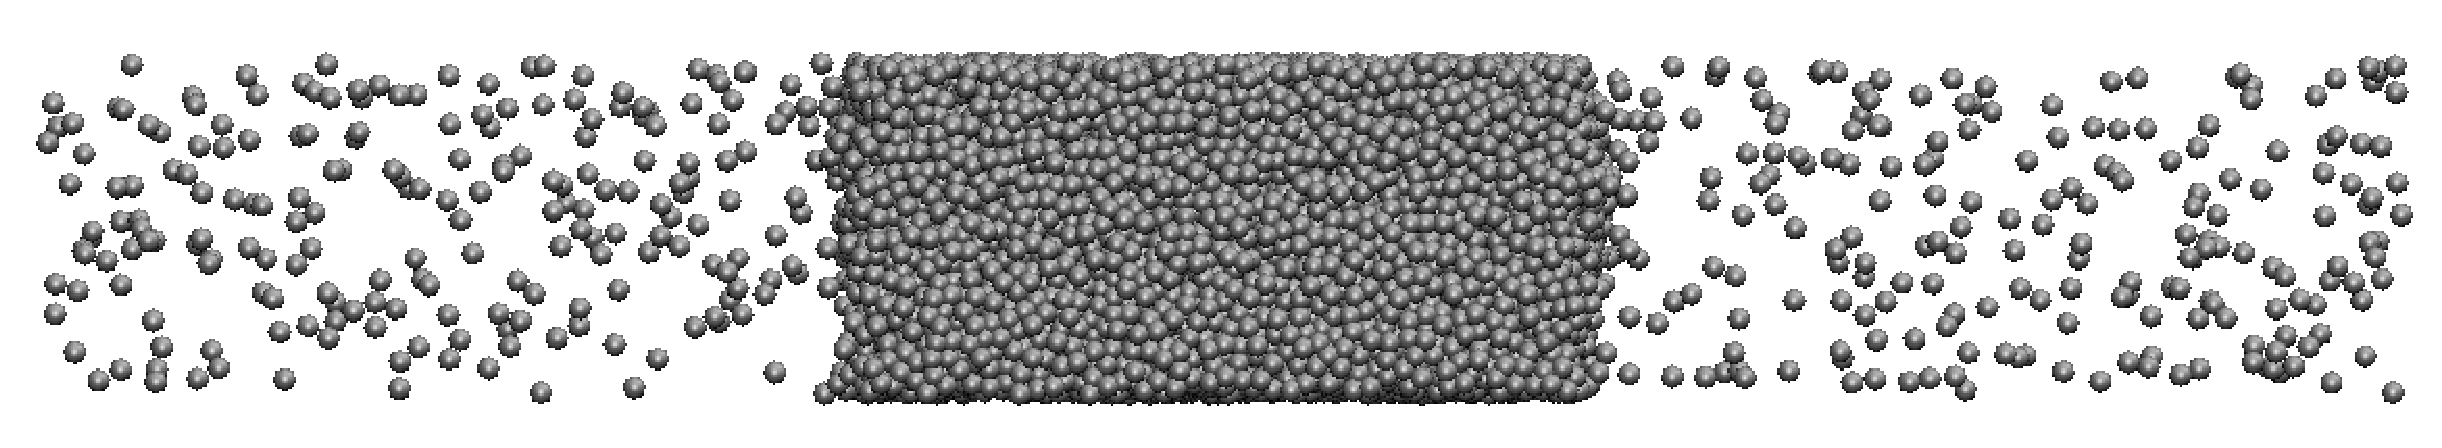
\includegraphics[width=0.9\textwidth]{fig/t0.85-n16000-rc07.5uni/confout.eps}
  \caption{The snapshot of the 16000 Lennard-Jones particle system at
    $T^\ast=0.85$ with a uniform cut-off radius of $r_c^\ast = 7.5$.}
  \label{fig:tmp1}
\end{figure}

\begin{figure}
  \centering
  % \includegraphics[]{fig/t0.85-n16000-rc07.5uni/confout-02.eps}
  \includegraphics[]{fig/t0.85-n16000-rc07.5uni/error.uniform.eps}
  \caption{The error distribution of the 16000 Lennard-Jones particle
    system at $T^\ast=0.85$ with a uniform cut-off radius of $r_c^\ast
    = 7.5$.}
  \label{fig:tmp2}
\end{figure}

% \begin{figure}
%   \centering
%   \includegraphics[]{fig/t0.85-n16000-adapt-e0.0045-extend/rcut.adapt.eps}
%   \caption{The adapted cut-off radius of the 16000 Lennard-Jones
%     particle system at $T^\ast=0.85$.}
%   \label{fig:tmp3}
% \end{figure}


% \begin{figure}
%   \centering
%   \includegraphics[]{fig/t0.85-n16000-adapt-e0.0045-extend/error.adapt.eps}
%   \caption{The error distribution of the adaptive-cut-off 16000
%     Lennard-Jones particle system at $T^\ast=0.85$.}
%   \label{fig:tmp4}
% \end{figure}


% \begin{figure}
%   \centering
%   \includegraphics[]{fig/t0.85-n16000-fcorr-rc07.5-feq0200/fcorr.eps}
%   \caption{The correction force simulation of the 16000 Lennard-Jones
%     particle system at $T^\ast=0.85$.}
%   \label{fig:tmp3}
% \end{figure}


% \begin{figure}
%   \centering
%   \includegraphics[]{fig/t0.85-n16000-fcorr-rc07.5-feq0200/error.fcorr.eps}
%   \caption{The correction force simulation of the adaptive-cut-off 16000
%     Lennard-Jones particle system at $T^\ast=0.85$.}
%   \label{fig:tmp4}
% \end{figure}


\begin{figure}
  \centering
  % \includegraphics[scale=1]{fig/t0.85-n16000-rc07.5uni/confout-02.eps}
  \includegraphics[]{fig/t0.85-n16000-adapt-e0.0045-extend/rcut.and.error.eps}
  \caption{The correction force simulation of the 16000 Lennard-Jones
    particle system at $T^\ast=0.85$.}
  \label{fig:tmp3}
\end{figure}

\begin{figure}
  \centering
  % \includegraphics[scale=1]{fig/t0.85-n16000-rc07.5uni/confout-02.eps}
  \includegraphics[]{fig/t0.85-n16000-fcorr-rc07.5-feq0200/fcorr.and.error.eps}
  \caption{The correction force simulation of the 16000 Lennard-Jones
    particle system at $T^\ast=0.85$.}
  \label{fig:tmp4}
\end{figure}




\begin{figure}
  \centering
  \includegraphics[width=0.49\textwidth]{fig/converge/t0.70.eps} 
  \includegraphics[width=0.49\textwidth]{fig/converge/t0.85.eps} 
  \includegraphics[width=0.49\textwidth]{fig/converge/t1.10.eps} 
  \includegraphics[width=0.49\textwidth]{fig/converge/t1.20.eps} 
  \caption{normal words}
  \label{fig:tmp5}
\end{figure}

\begin{figure}
  \centering
  \includegraphics[width=0.49\textwidth]{fig/converge/tension.t0.70.eps} 
  \includegraphics[width=0.49\textwidth]{fig/converge/tension.t0.85.eps} 
  \includegraphics[width=0.49\textwidth]{fig/converge/tension.t1.10.eps} 
  \includegraphics[width=0.49\textwidth]{fig/converge/tension.t1.20.eps} 
  \caption{normal words}
  \label{fig:tmp6}
\end{figure}


\subsection{Collision of nanoscale Lennard-Jones clusters}
\label{sec:tmp2.2}

In this section, we test how the adaptive cut-off method and the force
correction method work in a dynamical problem: collision of nanoscale
Lennard-Jones clusters. Two initial Lennard-Jones clusters, denoted by
$A$ and $B$, are setup in the simulation box, each of which contains
the same number of particles $N_A = N_B = 10792$, with a diameter of
$d^\ast\approx 27$. The initial velocity of the clusters are $\v u_A =
\frac12(u, 0, 0)$ and $\v u_B = -\frac12(u, 0, 0)$, see
Fig. \ref{fig:tmp7}. The impact parameter $D$ is defined by the $z$
corrdinate difference between the center of mass (COM) of the
clusters. The unitless impact factor defined by
\begin{align}
  x = \frac D d
\end{align}
is used to measure how far off-center the collision happens. If $x =
0$ the collision is head-on, while $x=1$ the collision is avoided.
Ref. \cite{kalweit2006collision} investigated a board range
combination of velocity $u$ and impact factor $x$, and identified
three major collision modes: the coalescence, the streching seperation
and the shattering. The major modes were further classified into a
series submodes. In this paper, we want to study the how the collision
properties of interests are affected by the force calculation
precision, therefore, we will NOT investigate a broad range of
parameters, but focus on one special case: $u^\ast = 2.2$ and $x =
0.6$, where poor precision of force calculation will lead to wrong
major collision modes.

In the top two plots of Fig. \ref{fig:tmp9}, we present the trajectory
of cluster $A$ and COM distance between the two clusters.  Three
different cut-off radii of uniform cut-off simulation are considered.
In this case the two clusters collide and form one rotating cluster.
It is obvious that the trajectory of $r_c^\ast = 2.5$ is completely
wrong: two clusters finally seperate. The $r_c^\ast = 5.0$ trajectory
is reasonably good, but the COM distance converges only when $r_c^\ast
= 7.5$. This means the precision of force calculation is crucial in
the study of collision dynamics.

The RMS force error of $r_c^\ast = 5.0$ uniform cut-off simulation,
the distribution of adaptive cut-off simulation and the magnitude of
the correction force are plotted in Fig. \ref{tmp:fig8}.  The
configuration of the two clusters (colored in gray and yellow) are
presented on the top for reference. The same as the liquid-vapor
equilibrium simulation, the error of the force located at the
interfacial region, namely the boundary of the clusters. Inside and
outside the clusters, the force error is much lower.  The maximum
cut-off used in the adaptive cut-off simulation is 5.0, which follows
the maximum RMS force error perfectly. The maximum cut-off region is
much border than the maximum error region, because it is refined by
twice to keep track of the possible moving of the clusters.  The
cut-off radius in the force correction simulation is 2.5, although
using such a small cut-off radius, the collision is in the right mode,
see also Fig. \ref{tmp:fig9}. The maximum of the correction force also
following the boundary of the colliding clusters, wheras in the interial
region of the clusters, the correction force is neglectable. 

The angular velocity is presented in the left plot of
Fig. \ref{tmp:fig10}. The force correction result is not as precise as
other simulations excluding uniform $r_c = 2.5$ simulation. This
because the correction force is not precise because it is calculated
every \recheck{aaa} steps. In the right plot of Fig. \ref{tmp:fig10},
the angular moment, which should be preserved is presented. All
uniform simulations preserved the angular moment perfectly. The
angular moment of the adaptive cut-off simulation, which does not
precisly preserve the Newton's third law, shows deviation but is still
around the correct value. However, the angular moment of the force
correction simulation flies away from the the correct value by 1 \% at
$t^\ast = 130$.


\begin{figure}
  \centering
  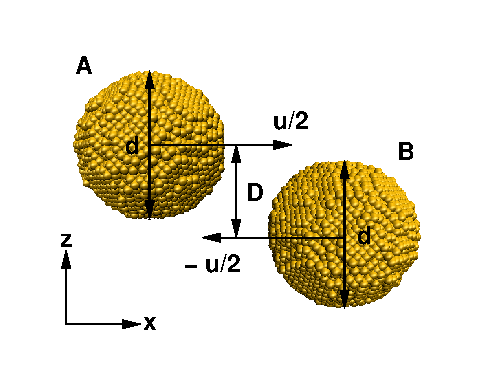
\includegraphics[]{fig/collision-init/init.2.eps}
  \caption{normal words}
  \label{fig:tmp7}
\end{figure}


\begin{figure}
  \centering
  \includegraphics[width=0.49\textwidth]{fig/trajs.eps}
  \includegraphics[width=0.49\textwidth]{fig/dists.eps}
  \caption{normal words}
  \label{fig:tmp9}
\end{figure}



\begin{figure}
  \centering
  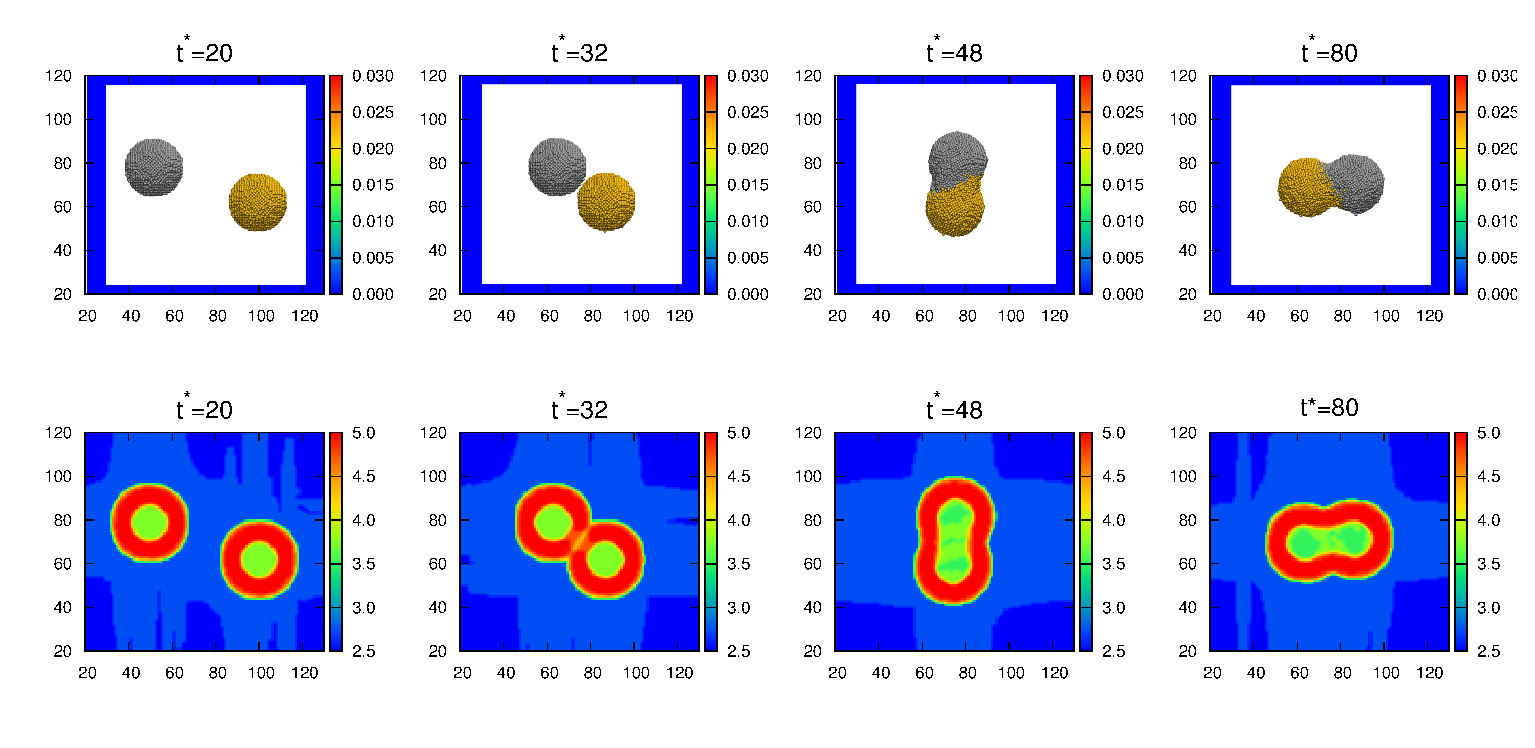
\includegraphics[width=0.90\textwidth]{fig/error-rcut-ball.eps} 
  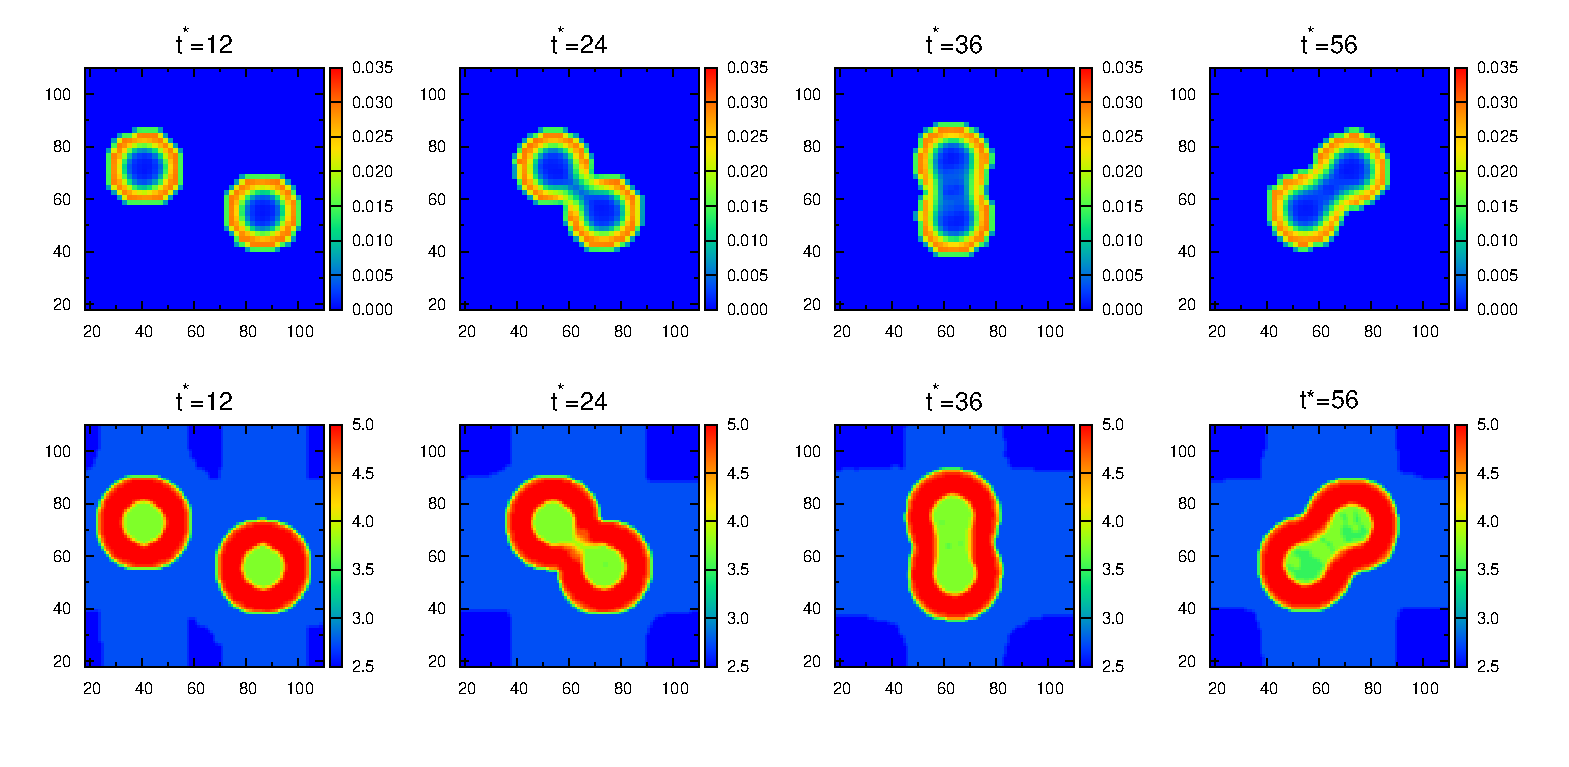
\includegraphics[width=0.90\textwidth]{fig/error-rcut.eps}
  \caption{normal words}
  \label{fig:tmp8}
\end{figure}

\begin{figure}
  \centering
  \includegraphics[width=0.49\textwidth]{fig/wy.eps}
  \includegraphics[width=0.49\textwidth]{fig/ly.eps}
  \caption{normal words}
  \label{fig:tmp10}
\end{figure}


% \newpage

% \bibliography{ref}{}
% \bibliographystyle{unsrt}


\end{document}
